\chapter{Regole del gioco}\label{chapter:background}

In questo capitolo, verrà presentata una panoramica delle basi teoriche e concettuali, in particolare sui giochi di carte collezionabili, soffermandosi su \emph{Magic: The Gathering}. Esploreremo le regole fondamentali che governano il gioco, suddividendole in concetti chiave e zone di gioco. Successivamente, verrà fornita un'introduzione su come leggere una carta di Magic, comprendendo le informazioni essenziali presenti su di essa. Inoltre, si esaminerà il concetto di motore di regole all'interno del contesto di Magic: The Gathering, con un focus particolare sul caso d'uso di Forge e il suo impatto nel giocare e comprendere il gioco.

\section{\textit{Magic The Gathering}}\label{sec:magic_the_gathering}
I giochi di carte collezionabili (GCC) sono un tipo di gioco di carte in cui i giocatori creano il proprio mazzo utilizzando una vasta gamma di carte disponibili, ognuna con caratteristiche e abilità uniche. Questi giochi combinano strategia, collezionismo e competizione, offrendo un'esperienza di gioco dinamica e coinvolgente. Tra i vari GCC, \emph{Magic: The Gathering} (anche detto semplicemente \emph{MtG} o \emph{Magic})  è il più longevo e popolare, lanciato nel 1993 da \emph{Wizards of the Coast} e creato dal matematico Richard Garfield.

\emph{Magic} è un gioco di strategia in cui due o più giocatori si sfidano utilizzando mazzi di carte personalizzati, con l'obiettivo di ridurre i punti vita dell'avversario a zero. Ogni giocatore inizia con un mazzo composto da almeno 60 carte, che possono essere di diversi tipi, tra cui creature, incantesimi, artefatti e terre.

Il gioco si svolge in turni, durante i quali i giocatori possono pescare carte, mettere in gioco terre, evocare creature e lanciare incantesimi o abilità. Le terre forniscono mana, la risorsa necessaria per giocare le altre carte. Ogni carta ha un costo di mana, indicato nell'angolo superiore destro, che rappresenta la quantità di mana necessaria per giocarla.

Le creature possono attaccare gli avversari o difendere il proprio giocatore dagli attacchi nemici. Ogni creatura ha due valori numerici: la forza, che indica la quantità di danno che può infliggere, e la costituzione, che indica la quantità di danno che può subire prima di essere distrutta.

Gli incantesimi e gli artefatti, invece, hanno effetti variabili che possono influenzare il campo di battaglia, le creature, i giocatori o altre carte in gioco. Questi effetti possono essere temporanei o permanenti, e possono avere un impatto significativo sull'andamento della partita.

\subsection{Come leggere una carta di \emph{Magic}}\label{subsec:mtg_cards}
Una carta di \emph{Magic} presenta diverse componenti chiave che forniscono informazioni sulle sue caratteristiche e funzioni. Di seguito è riportata una descrizione delle principali componenti di una carta, con l'immagine nella Figura \ref{fig:one} come esempio\footnote{ Sezione ``Part of a Card" delle regole comprensive \cite{mtg-comp-rules}}:



\begin{figure}[ht]
	\centering
        \begin{tikzpicture}
            \node[anchor=south west,inner sep=0] (image) at (0,0) {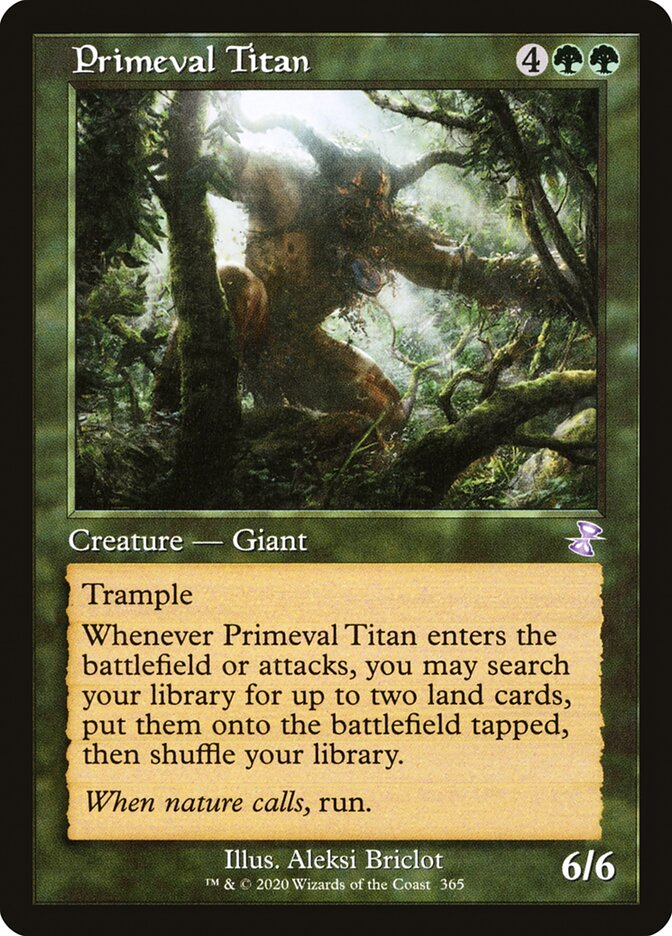
\includegraphics[width=0.5\textwidth]{Immagini/tsr-365-primeval-titan.jpg}};
            \begin{scope}[x={(image.south east)},y={(image.north west)}]
                \fill[red!50, opacity=0.5] (0.07,0.935) circle (0.27cm);
                \node [black, font=\Large] at (0.07,0.935) {a};
                \fill[red!50, opacity=0.5] (0.72, 0.94) circle (0.27cm);
                \node [black, font=\Large] at (0.72, 0.94) {b};
                \fill[red!50, opacity=0.5] (0.6, 0.6)  circle (0.27cm);
                \node [black, font=\Large] at (0.6, 0.6) {c};
                \fill[red!50, opacity=0.5] (0.07,0.42) circle (0.27cm);
                \node [black, font=\Large] at (0.07,0.42) {d};
                \fill[red!50, opacity=0.5] (0.5, 0.425)  circle (0.27cm);
                \node [black, font=\Large] at (0.5, 0.425) {e};
                \fill[red!50, opacity=0.5] (0.6, 0.15)  circle (0.27cm);
                \node [black, font=\Large] at (0.6, 0.15) {f};
                \fill[red!50, opacity=0.5] (0.25, 0.07)  circle (0.27cm);
                \node [black, font=\Large] at (0.25, 0.07) {g};
                \fill[red!50, opacity=0.5] (0.8, 0.07)  circle (0.27cm);
                \node [black, font=\Large] at (0.8, 0.07) {h};

            \end{scope}
        \end{tikzpicture}
	\caption{Carta di \emph{Magic the Gathering} con layout vintage}
	\label{fig:one}
\end{figure}




\begin{enumerate}[label=\alph*.]
    \item \textbf{Nome}: nella parte superiore della carta, si trova il nome univoco della carta, permettendo ai giocatori di identificarla facilmente e distinguerla dalle altre. 
    
    \item \textbf{Costo di mana}: nell'angolo superiore destro della carta, è presente il costo di mana necessario per giocare la carta, composto da simboli che rappresentano i diversi colori di mana (bianco, blu, nero, rosso e verde) e/o un numero che indica la quantità di mana generico richiesta.
    
    \item \textbf{Illustrazione}: al centro della carta, vi è un'illustrazione che rappresenta la carta e contribuisce all'ambientazione e all'atmosfera del gioco. 
    
    \item \textbf{Tipo di carta}: appena sotto l'illustrazione, si trova il tipo di carta, che può essere creatura, incantesimo, artefatto, terra, o una combinazione di questi. Il tipo di carta determina le regole generali che si applicano alla carta e il modo in cui può essere utilizzata durante il gioco. 
    
    \item \textbf{Sottotipo}: alcune carte hanno anche un sottotipo, che fornisce ulteriori informazioni sulla carta e sulle sue interazioni con altre carte. Ad esempio, una creatura potrebbe avere un sottotipo come ``Gigante" o ``Mago". 
    
    \item \textbf{Testo delle abilità}: nella parte centrale della carta, si trova il testo delle abilità, che descrive gli effetti e le regole specifiche della carta. Questo testo può includere parole chiave (Keywords), effetti che si attivano quando la carta entra in gioco, o abilità attivabili che richiedono un costo specifico per essere utilizzate. Può contenere anche un testo narrativo relativo al soggetto dell'illustrazione.
    
    \item \textbf{Informazioni legali e di collezionismo}: nella parte inferiore della carta, si trovano informazioni legali, il numero di collezionismo e l'edizione a cui appartiene la carta. Queste informazioni sono utili per i collezionisti e per determinare l'ammissibilità delle carte nei diversi formati di gioco. 
    
    \item \textbf{Forza/Costituzione}: per le carte creature, nella parte inferiore destra della carta, si trovano due numeri separati da una barra (/). Il primo numero indica la forza della creatura, ovvero la quantità di danno che può infliggere in combattimento\footnote{Questo argomento sarà approfondito nella Sezione \ref{subsec:mtg_turns} -- Parti del turno}, mentre il secondo numero rappresenta la costituzione, che indica la quantità di danno che la creatura può subire prima di essere distrutta.     
\end{enumerate}


\subsection{Le zone di gioco}\label{subsec:mtg_zones}
In \emph{Magic}, il tavolo di gioco si divide in diverse zone, ognuna delle quali ha uno scopo specifico e delle regole associate. Di seguito è riportata una descrizione delle principali zone di gioco\footnote{ Sezione ``Zones" delle regole comprensive \cite{mtg-comp-rules}}:


\begin{figure}[ht]
	\centering
        \begin{tikzpicture}
            \node[anchor=south west,inner sep=0] (image) at (0,0) {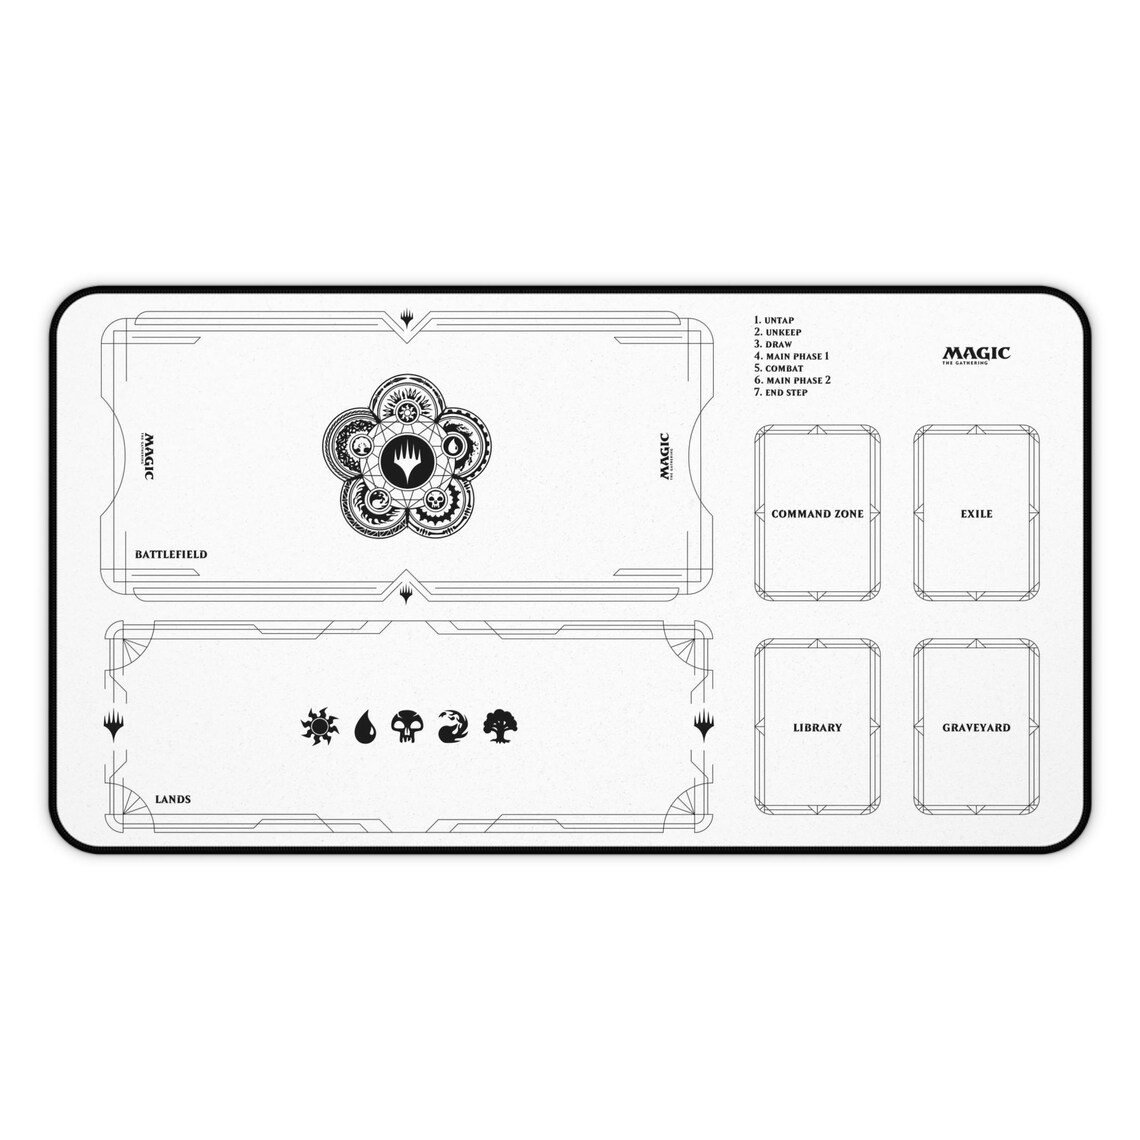
\includegraphics[width=\textwidth, trim= 0 200 0 200, clip]{Immagini/card_zones.jpg}};
            \begin{scope}[x={(image.south east)},y={(image.north west)}]
                \fill[red!50, opacity=0.5] (0.69,0.22) circle (0.27cm);
                \node [black, font=\Large] at (0.69,0.22) {a};
                \fill[red!50, opacity=0.5] (0.5, 0.07) circle (0.27cm);
                \node [black, font=\Large] at (0.5, 0.07) {b};
                \fill[red!50, opacity=0.5] (0.355,0.52) circle (0.27cm);
                \node [black, font=\Large] at (0.355,0.52) {c};
                \fill[red!50, opacity=0.5] (0.5, 0.92)  circle (0.27cm);
                \node [black, font=\Large] at (0.5, 0.92) {d};
                \fill[red!50, opacity=0.5] (0.825, 0.22)  circle (0.27cm);
                \node [black, font=\Large] at (0.825, 0.22) {e};
                \fill[red!50, opacity=0.5] (0.825, 0.5)  circle (0.27cm);
                \node [black, font=\Large] at (0.825, 0.5) {f};
                \fill[red!50, opacity=0.5] (0.69, 0.50)  circle (0.27cm);
                \node [black, font=\Large] at (0.69, 0.50) {g};

            \end{scope}
        \end{tikzpicture}
	\caption{Layout tipico del tavolo di gioco di \emph{Magic} (uno per giocatore)}
	\label{fig:two}
\end{figure}

\begin{enumerate}[label=\alph*.]
    \item \textbf{Grimorio (Library)}: Il grimorio è il mazzo di carte di un giocatore, disposto in un ordine casuale all'inizio della partita. I giocatori pescano carte dal loro grimorio durante il gioco. Non è consentito guardare le carte nel proprio grimorio o cambiarne l'ordine, a meno che una carta o un'abilità non lo consenta esplicitamente.
    
    \item \textbf{Mano (Hand)}: La mano di un giocatore è composta dalle carte che ha pescato ma non ha ancora giocato. I giocatori possono avere un massimo di sette carte in mano alla fine del loro turno, a meno che una carta o un'abilità non modifichi questo limite. Le carte in mano sono nascoste agli avversari.
    
    \item \textbf{Campo di battaglia (Battlefield)}: Il campo di battaglia è la zona di gioco in cui si trovano i permanenti, come creature, artefatti, incantesimi e terre. Questi permanenti sono visibili a tutti i giocatori e interagiscono tra loro secondo le regole del gioco e le abilità delle singole carte.
    
    \item \textbf{Pila (Stack)}: La pila è la zona in cui vengono messe le magie e le abilità innescate o attivate che sono state lanciate o attivate ma non si sono ancora risolte. La pila funziona secondo il principio ``ultimo entrato, primo uscito" (Last In, First Out - LIFO), il che significa che la carta o l'abilità aggiunta per ultima alla pila sarà la prima a risolversi.
    
    \item \textbf{Cimitero (Graveyard)}: Il cimitero è la zona di gioco in cui vengono messe le carte che sono state utilizzate, distrutte, scartate o che hanno risolto i loro effetti. Il cimitero è visibile a tutti i giocatori e alcune carte o abilità possono interagire con le carte nel cimitero.
    
    \item \textbf{Zona di esilio (Exile)}: La zona di esilio è una zona di gioco separata in cui vengono messe le carte rimosse dal gioco a causa di effetti o abilità specifiche. Le carte in esilio sono generalmente considerate fuori dal gioco e non possono essere utilizzate, a meno che una carta o un'abilità non consenta esplicitamente di interagire con le carte esiliate.
    
    \item \textbf{Zona di comando (Command zone)}: La Command Zone è una zona di gioco utilizzata in alcuni formati di Magic, come il Commander. In questi formati, i giocatori hanno una carta "comandante" che inizia il gioco nella Command Zone e può essere giocata da lì.
\end{enumerate}

\subsection{Parti del turno}\label{subsec:mtg_turns}

Ogni turno procede secondo la stessa sequenza. Quando inizia una nuova fase o sottofase, ogni abilità innescata che si verifica durante quella sottofase si innesca e viene messa in pila. Il giocatore attivo (il giocatore di cui è il turno) può iniziare a lanciare magie e attivare abilità, seguito da ogni altro giocatore in ordine di turno. Quando tutti i giocatori decidono di non fare più nulla e non c'è nulla in pila in attesa di risolversi, la partita avanzerà alla sottofase successiva\footnote{ Sezione ``Turn Structure" delle regole comprensive \cite{mtg-comp-rules}}.

\subsubsection{Fase iniziale} 
\begin{enumerate}[label=\alph*.] 
\item Sottofase di \emph{STAP (Untap)}: STAPpato/TAPpato rappresentano la condizione di una carta, rispettivamente la capacità e incapacità della stessa di essere utilizzata per determinate azioni durante il gioco. Si STAPpano tutti i permanenti TAPpati del giocatore di turno. Nel primo turno di gioco, se non si hanno permanenti, questa sottofase viene saltata%\footnote{TAP e STAP si riferiscono allo stato di un permanente. Un permanente TAPpato è stato utilizzato per un'azione o un effetto, mentre un permanente STAPpato è disponibile per essere utilizzato.}
. Non è possibile lanciare magie o attivare abilità durante questa sottofase. 
\item Sottofase di \emph{Mantenimento (Upkeep)}: I giocatori possono lanciare istantanei e attivare abilità. Questa parte del turno è menzionata su numerose carte. Se un'abilità deve verificarsi solo una volta per turno, precisamente all'inizio, si innescherà “all'inizio del mantenimento” del giocatore di turno. 
\item Sottofase di \emph{Acquisizione (Draw)}: Il giocatore di turno deve pescare una carta dal proprio grimorio. Il giocatore che gioca per primo in una partita a due giocatori salta la sottofase di acquisizione nel suo primo turno per compensare il vantaggio di giocare per primo. Successivamente, i giocatori possono lanciare istantanei e attivare abilità. 
\end{enumerate}

\subsubsection{Prima fase principale} Il giocatore di turno può lanciare un qualsiasi numero di stregonerie, istantanei, creature, artefatti, incantesimi e attivare abilità. È possibile giocare una terra in questa fase, ma si ricorda che si può giocarne soltanto una per turno. Gli avversari possono lanciare istantanei e attivare abilità.


\subsubsection{Fase di Combattimento}
\begin{enumerate}[label=\alph*.]
    
    \item Sottofase di dichiarazione delle creature attaccanti: Il giocatore di turno decide quali delle proprie creature STAPpate (anche nessuna) attaccheranno e quale giocatore colpiranno. Le creature attaccanti vengono TAPpate. Successivamente, i giocatori possono lanciare istantanei e attivare abilità.
    
    \item Sottofase di dichiarazione delle creature bloccanti: L'avversario decide quali delle proprie creature STAPpate (anche nessuna) bloccheranno le creature attaccanti del giocatore di turno. Se più di una creatura blocca la stessa creatura attaccante, il giocatore di turno deve ordinare le creature bloccanti per mostrare quale subirà il danno per prima, quale per seconda e così via. In seguito, i giocatori possono lanciare istantanei e attivare abilità.
    
    \item Sottofase di danno da combattimento: Ogni creatura attaccante o bloccante che si trova ancora sul campo di battaglia assegna il proprio danno da combattimento al giocatore in difesa (se stava attaccando quel giocatore e non è stata bloccata), alla creatura o alle creature che la stanno bloccando. Se più di una creatura blocca la stessa creatura attaccante, il giocatore di turno deve dividere il danno da combattimento tra di esse, assegnando almeno danno sufficiente a distruggere la prima creatura bloccante, prima di poter assegnare il danno rimanente alla creatura successiva e così via. Una volta che i giocatori hanno deciso come le creature che controllano infliggeranno il loro danno da combattimento, tutto il danno viene inflitto contemporaneamente. Successivamente, i giocatori possono lanciare istantanei e attivare abilità.
    
\end{enumerate}

\subsubsection{Seconda fase principale}
La seconda fase principale è simile alla prima. Il giocatore di turno può lanciare magie di tutti i tipi e attivare abilità, mentre gli avversari possono soltanto lanciare istantanei e attivare abilità. È possibile giocare una terra in questa fase, se non è stata già giocata nella prima fase principale.

\subsubsection{Fase finale}
\begin{enumerate}[label=\alph*.]
    \item Sottofase finale: Le abilità che si innescano “all'inizio della sottofase finale” del giocatore di turno vengono messe in pila. I giocatori possono lanciare istantanei e attivare abilità.
    \item Sottofase di cancellazione: Se il giocatore di turno ha più di sette carte in mano, deve scegliere e scartare carte fino ad arrivare a sette. Successivamente, viene rimosso tutto il danno dalle creature e gli effetti “fino alla fine del turno” terminano. Nessuno può lanciare istantanei o attivare abilità, a meno che non si inneschi un'abilità durante questa sottofase.
\end{enumerate}


\section{Cos'è un motore di regole (Rule Engine)}\label{sec:rule_engine}
Non esiste una definizione consolidata di Rule Engine nel contesto della digitalizzazione dei giochi di carte e da tavolo. Tuttavia, nel contesto dello sviluppo software, un rule engine è un componente software che permette di separare la logica di business dall'implementazione tecnica di un'applicazione. Questo strumento consente di definire le regole di applicazione in un formato dichiarativo, rendendo la gestione della logica complessa del sistema più flessibile e manutenibile. Le regole, espresse in termini di condizioni e azioni, possono essere valutate dinamicamente durante l'esecuzione dell'applicazione, consentendo una personalizzazione del comportamento senza la necessità di modificare il codice sorgente. Questo approccio favorisce la separazione delle responsabilità e promuove una maggiore adattabilità del sistema alle mutevoli esigenze del business \cite{fowler-rule-engine}.
Per i videogiochi tradizionali, l'attenzione è solitamente posta sul motore di gioco, che include il motore di rendering, il motore audio, il motore fisico, gli strumenti di intelligenza artificiale e altri middleware simili, come moduli di animazione, librerie 2D e 3D e strumenti di authoring. Tuttavia, nei giochi di carte e da tavolo, come \emph{Magic}, le regole del gioco sono estremamente importanti e richiedono un approccio diverso per gestire la logica del gioco.\linebreak

Ecco alcuni elementi chiave di un rule engine:

\begin{enumerate}[label=\alph*.]
    \item \textit{Gestione delle regole}: Un rule engine consente di definire, memorizzare e organizzare le regole aziendali in un formato strutturato. Le regole possono essere definite utilizzando un linguaggio specifico del dominio o attraverso un'interfaccia utente grafica, a seconda del rule engine utilizzato.

    \item \textit{Valutazione delle regole}: Il rule engine valuta le regole in base ai dati forniti e determina quali regole sono attivate o soddisfatte. Questo processo di valutazione può coinvolgere la valutazione di condizioni logiche, la combinazione di regole e la gestione delle priorità delle regole.

    \item \textit{Esecuzione delle azioni}: Una volta che le regole sono attivate, il rule engine esegue le azioni associate a ciascuna regola. Le azioni possono includere l'aggiornamento dei dati, l'avvio di processi aziendali, l'invio di notifiche o qualsiasi altra operazione definita nell'ambito delle regole.
    
    
    \item \textit{Flessibilità e aggiornabilità}: I rule engine sono progettati per essere flessibili e facilmente aggiornabili. Le regole possono essere modificate o aggiunte senza dover modificare il codice dell'applicazione principale, il che consente una maggiore agilità aziendale e una rapida risposta ai cambiamenti nei requisiti aziendali.

    \item \textit{Monitoraggio e tracciabilità}: I rule engine spesso forniscono strumenti per il monitoraggio delle regole attivate e delle azioni eseguite. Questo consente agli sviluppatori e agli amministratori di sistema di tracciare il comportamento del sistema e di risolvere eventuali problemi o discrepanze.
\end{enumerate}


\begin{table}[ht]
	\centering
	\resizebox{0.99\linewidth}{!}{
		\begin{tabular}{||c||c|c|c|c|c||}
			\hhline{|t:=:t:+=====:t|}
			Nome &\phantom{00}DesktopOS\phantom{00}&\phantom{00}Linguaggio\phantom{00}&\phantom{00}Carte Implementate\phantom{00}&\phantom{00}Open Source\phantom{00}&\phantom{00}Scripted\phantom{00} \\
			\hhline{|:=::=====:|}
			Forge \cite{forge_repo}&Any (Java)&Java&27.474&\checkmark&\checkmark \\
			\hhline{||-||-----||}
   			MtG Arena (GRE) \cite{mtg-gre}&Any&C++ \& CLISP&10.199 (MtgA) & &\checkmark   \\
			\hhline{||-||-----||}
               MtG Online&Windows&C++ & Tutte (escluse edizioni scherzo)& & n.d.  \\
			\hhline{||-||-----||}
            Xmage&Any (Java)&Java&17.218&\checkmark &  \\
			\hhline{||-||-----||}
            Incantus&Any (Python)&Python&2.583&\checkmark & \checkmark \\
			\hhline{||-||-----||}
            Magarena&Any (Java)&Java&11.854&\checkmark & \checkmark \\
			\hhline{||-||-----||}
            BotArena&Windows&C++&10.744&\checkmark &  \\
			\hhline{||-||-----||}
            Multiverse&Any&Java&1.500&  & \checkmark \\
			\hhline{||-||-----||}
            Wagic&Any&C++&24.570& \checkmark  & \checkmark \\
			\hhline{||-||-----||}
            \hhline{|b:=:b:+=====:b|}
		\end{tabular}
	}
	\vspace*{2mm}
	\caption{Lista dei Rule Engine per \emph{Magic the Gathering}}
	\label{tab:mtg_engine}
\end{table}

\section{Caso d'uso: Forge}\label{sec:forge_rule_engine}
Forge è un rule engine open-source specificamente progettato per il gioco di carte collezionabili \emph{Magic}. Il Rule Engine Forge consente agli sviluppatori e agli appassionati di creare e simulare partite di \emph{Magic}, gestendo le complesse regole e interazioni del gioco in modo automatico e coerente. Grazie alla sua architettura modulare e alla sua vasta base di utenti, Forge è diventato uno strumento popolare per lo sviluppo di applicazioni e simulatori basati su \emph{Magic}.\linebreak


Le principali caratteristiche di Forge sono:

\begin{enumerate}[label=\alph*.]
    \item \textbf{Implementazione delle regole di \emph{Magic}}: Forge implementa le regole di Magic: The Gathering, gestendo le interazioni tra carte, abilità, zone di gioco e turni. Ciò consente agli sviluppatori di concentrarsi sull'interfaccia utente e sulle funzionalità specifiche del loro progetto, senza dover reinventare la gestione delle regole di \emph{Magic}.

    \item \textbf{Aggiornamenti continui}: La comunità di Forge lavora costantemente per aggiornare il rule engine con le nuove carte e le modifiche alle regole di \emph{Magic}. Ciò garantisce che Forge rimanga aggiornato con le ultime espansioni e cambiamenti nel gioco.
    
    \item \textbf{Modalità di gioco supportate}: Forge supporta diverse modalità di gioco, tra cui partite singole, multiplayer, draft e sealed. Ciò consente agli sviluppatori di creare applicazioni che offrono un'ampia gamma di esperienze di gioco per i giocatori di \emph{Magic}.
    
    \item \textbf{Intelligenza artificiale}: Forge include un'intelligenza artificiale (AI) che consente ai giocatori di sfidare avversari controllati dal computer. % L'AI di Forge è progettata per emulare il comportamento di un giocatore umano e può essere ulteriormente personalizzata e migliorata dagli sviluppatori.
    
    \item \textbf{Piattaforme supportate}: Forge è scritto in Java, il che lo rende compatibile con una vasta gamma di piattaforme, tra cui Windows, macOS, Linux e dispositivi mobili. Questa compatibilità multi-piattaforma consente agli sviluppatori di creare applicazioni di \emph{Magic} che possono essere giocate su una varietà di dispositivi.

\end{enumerate}
